\documentclass{article}

\usepackage{amsmath,amssymb}
\usepackage{graphicx}
\usepackage{array}
\usepackage[margin=1in]{geometry}
\usepackage{dsfont}

% ===== This makes my \affil cmnd work.
\usepackage[affil-it]{authblk}


% ===== This makes my environments work switching llncs to article.
\newtheorem{theorem}{Theorem}[section]
\newtheorem{lemma}[theorem]{Lemma}
\newtheorem{proposition}[theorem]{Proposition}
\newtheorem{corollary}[theorem]{Corollary}

\newenvironment{proof}[1][Proof]{\begin{trivlist}
\item[\hskip \labelsep {\bfseries #1}]}{\end{trivlist}}
\newenvironment{definition}[1][Definition]{\begin{trivlist}
\item[\hskip \labelsep {\bfseries #1}]}{\end{trivlist}}
\newenvironment{example}[1][Example]{\begin{trivlist}
\item[\hskip \labelsep {\bfseries #1}]}{\end{trivlist}}
\newenvironment{remark}[1][Remark]{\begin{trivlist}
\item[\hskip \labelsep {\bfseries #1}]}{\end{trivlist}}

\newcommand{\qed}{\nobreak \ifvmode \relax \else
      \ifdim\lastskip<1.5em \hskip-\lastskip
      \hskip1.5em plus0em minus0.5em \fi \nobreak
      \vrule height0.75em width0.5em depth0.25em\fi}

% ===== For \algorithm. Is this a decent idea?
\usepackage[lined,boxed,ruled,vlined]{algorithm2e}

% ===== For \mathscr
\usepackage{mathrsfs}
\DeclareSymbolFontAlphabet{\mathrsfs}{rsfs}
\usepackage[mathscr]{eucal}


% ===== For \boldsymbol
\usepackage{amsbsy}

% ===== For \bm (bold math)
\usepackage{bm}

\usepackage{fixltx2e}
\MakeRobust{\overrightarrow}

% ===== For code snippets
\usepackage{courier}

% ==== Misha and Ning's Notation file =====
%% ----------------------------------------------------------------------
%% Definitions, Macros, Etc.
%% ----------------------------------------------------------------------

%% Hyper-linked References
\newcommand{\Sec}[1]{\hyperref[sec:#1]{\S\ref*{sec:#1}}} %section
\newcommand{\Eqn}[1]{\hyperref[eq:#1]{(\ref*{eq:#1})}} %equation
\newcommand{\Fig}[1]{\hyperref[fig:#1]{Figure~\ref*{fig:#1}}} %figure
\newcommand{\Tab}[1]{\hyperref[tab:#1]{Table~\ref*{tab:#1}}} %table
\newcommand{\Thm}[1]{\hyperref[thm:#1]{Theorem~\ref*{thm:#1}}} %theorem
\newcommand{\Lem}[1]{\hyperref[lem:#1]{Lemma~\ref*{lem:#1}}} %lemma
\newcommand{\Prop}[1]{\hyperref[prop:#1]{Property~\ref*{prop:#1}}} %property
\newcommand{\Cor}[1]{\hyperref[cor:#1]{Corollary~\ref*{cor:#1}}} %corollary
\newcommand{\Def}[1]{\hyperref[def:#1]{Definition~\ref*{def:#1}}} %definition
\newcommand{\Alg}[1]{\hyperref[alg:#1]{Algorithm~\ref*{alg:#1}}} %algorithm
\newcommand{\Ex}[1]{\hyperref[ex:#1]{Example~\ref*{ex:#1}}} %example

% Theorem-like constructs
%\newtheorem{example}[theorem]{Example}

% Blackboard fonts 
\newcommand{\Real}{\mathbb{R}}
\newcommand{\Cplx}{\mathbb{C}}
%% Transposes
\newcommand{\Tra}{^{\rm T}} % Transpose
\newcommand{\Cct}{^\dagger} % Complex conjugate transpose

%% Permutation index
\newcommand{\bfpp}{{\bf p}_n}

%% Matrix & Tensor Operations
\newcommand{\Circ}[1]{{\rm circ}\left( #1 \right)}
\newcommand{\Fold}[1]{{\rm fold}\left( #1 \right)}
\newcommand{\Unfold}[1]{{\rm unfold}\left( #1 \right)}
\newcommand{\Twist}[1]{{\rm twist}(\M{#1})}
\newcommand{\Squeeze}[1]{{\rm squeeze}(#1)}
\newcommand{\squeeze}{{\rm squeeze}}
\newcommand{\Mout}{\diamondsuit}
\newcommand{\circu}{ {\rm circ}}
\newcommand{\bcirc}{ {\rm circ}}
\newcommand{\vvec}{ {\rm vec}}

\newcommand{\mc}[1]{\mathcal{#1}}
\newcommand{\mb}[1]{\mathbb{#1}}
\newcommand{\mcr}[1]{\mathrsfs{#1}}

%% Element of complicated object that is surrounded by parens
\newcommand{\PE}[2]{\left( #1 \right)_{#2}}

%% Vector notation
\newcommand{\V}[1]{{\bm{\mathbf{\MakeLowercase{#1}}}}} % vector
\newcommand{\VE}[2]{\MakeLowercase{#1}_{#2}} % vector element

%% Matrix notation
\newcommand{\M}[1]{{\bm{\mathbf{\MakeUppercase{#1}}}}} % matrix
\newcommand{\Mhat}[1]{{\bm{\hat \mathbf{\MakeUppercase{#1}}}}} % matrix
\newcommand{\Mbar}[1]{{\bm{\bar \mathbf{\MakeUppercase{#1}}}}} % matrix
\newcommand{\ME}[2]{\MakeLowercase{#1}_{#2}} % matrix element
\newcommand{\MC}[2]{\V{#1}_{#2}}

%% Tensor notation
\newcommand{\T}[1]{\boldsymbol{\mathscr{\MakeUppercase{#1}}}} %tensor
\newcommand{\TLS}[2]{\M{#1}_{[#2]}} % lateral slice
\newcommand{\TFS}[2]{\M{#1}_{#2}} % frontal slice
\newcommand{\TT}[2]{\V{#1}_{#2}} % tube
\newcommand{\TE}[2]{\MakeLowercase{#1}_{#2}} % tensor element


%% Shortcuts
\newcommand{\TA}{\T{A}}
\newcommand{\TB}{\T{B}}
\newcommand{\TS}{\T{S}}
\newcommand{\TC}{\T{C}}
\newcommand{\TU}{\T{U}}
\newcommand{\TV}{\T{V}}
\newcommand{\TG}{\T{G}}

\newcommand{\Vu}{\V{u}}
\newcommand{\Vv}{\V{v}}
\newcommand{\Vq}{\V{q}}
\newcommand{\Vr}{\V{r}}
\newcommand{\Vp}{\V{p}}
\newcommand{\Vd}{\V{d}}
\newcommand{\Vz}{\V{z}}
\newcommand{\Vb}{\V{b}}
\newcommand{\Vg}{\V{g}}
\newcommand{\Vh}{\V{h}}
\newcommand{\MH}{\M{H}}
\newcommand{\MG}{\M{G}}
\newcommand{\MA}{\M{A}}
\newcommand{\MX}{\M{X}}
\newcommand{\MZ}{\M{Z}}
\newcommand{\MW}{\M{W}}
%\newcommand{\TD}{\T{D}}

\newcommand{\SaS}{{\mathcal S}}

\newcommand{\MGC}{\tilde{\MG}}

\newcommand{\Matlab}{{\sc Matlab}\xspace}
\newcommand{\matlab}{{\sc Matlab}\xspace}
\newcommand{\qtext}[1]{\quad\text{#1}\quad}

\newcommand{\matvec}{{\tt Vec}}
\newcommand{\fld}{{\tt Fold}}

\def \bK{\mathbf{K}}
\def \bF{\mathbf{F}}
\def \bD{\mathbf{D}}
\def \bB{\mathbf{B}}
\def \bA{\mathbf{A}}
\newcommand{\bDelta}{\boldsymbol{\Delta}}

%\newcommand{\bea}{\left[ \begin{array}}
%\newcommand{\eea}{ \end{array} \right]} 

\newcommand{\bftheta}{ {\boldsymbol \theta}}
\newcommand{\bfrho}{ {\boldsymbol \rho}}
\newcommand{\bfeta}{ {\boldsymbol \eta}}
\newcommand{\fft}{ \mbox{\tt fft} }
\newcommand{\ifft}{ \mbox{\tt ifft} }
\newcommand{\blkd}{\mbox{\tt blkdiag}}
\newcommand{\rshpT}{\mbox{\tt reshapeT}}
\newcommand{\F}[1]{\mathcal{F}\{#1\}}
\newcommand{\Fi}[1]{\mathcal{F}^{-1}\{#1\}}
\newcommand{\indep}{\perp\!\!\!\perp}

\usepackage{mathtools}
\DeclarePairedDelimiter{\ceil}{\lceil}{\rceil}
\DeclarePairedDelimiter{\floor}{\lfloor}{\rfloor}
\newcommand{\Var}{\text{Var}}
\newcommand{\E}{\text{E}}
\newcommand{\Cov}{\text{Cov}}



%%%% Dr. K's colored comments. 
\usepackage{color} 
\definecolor{blue}{rgb}{0,0,1}
\definecolor{red}{rgb}{1,0,0}
\definecolor{purple}{rgb}{1,0,1}
\newcommand\MEK[1]{\textcolor{red}{MEK: #1}}
\newcommand\EMK[1]{\textcolor{purple}{EMK: #1}}
\newcommand\SA[1]{\textcolor{blue}{SA: #1}}
\newcommand\red[1]{\textcolor{red}{#1}}
\begin{document}



Eric Kernfeld

Summary of Wilkinson's ``Parameter inference for stochastic kinetic models of bacterial gene regulation'', a book chapter in \cite{Bernardo2012}.

\begin{abstract}
In this paper, Wilkinson attempts to infer reaction rates for biochemical networks in a setting with discrete observations, missing data, and measurement error. He uses vague priors and likelihood-free MCMC methods within a Bayesian model. He runs four main simulations. The first three iterate through successively more difficult and realistic measurement models, and they show the approach can accurately infer three key reaction rates with a useful precision. The fourth studies a naive model, showing it leads to overconfident, incorrect inferences. All tests are conducted using synthetic data on only one vector of true parameters.

I plan to implement the method in Julia and reproduce the experiments. To honestly test the method, I need to do more simulations, too: what happens when the log-space mean of the prior is not near the true values, or when the true values are somewhere other than Wilkinson's choice? What happens when all the parameters are unknown, rather than just the three we are interested in?
\end{abstract}


\section{Introduction}
\subsection{Summary}
This paper develops tools to study bacterial behavior. There is a line of research modeling biochemical systems as continuous-time Markov jump processes, and this approach has physical motivation. The inherent stochasticity can also explain why three bacteria in similar environments may act differently. Much is known about biochemical network structure, but less about parameter values \cite{klipp2004inferring}, so within this area, Wilkinson's research fill a gap in parameter inference for Markov jump processes. The problem is difficult because in practice the data are partial, discrete-time, and noisy; for mathematical flexibility, his paper uses Bayesian inference and MCMC. The method is computationally intensive and excruciatingly serial, but it is accurate and shows potential for flexibility. Wilkinson's method or its variants may ultimately help reverse-engineer the regulatory networks that determine bacterial behavior and survival, though because of problems with scaling, it will probably be superseded by other research \footnote{Much of the alternative research Wilkinson cites is from his own research group, which seems to be trying out every available strategy on this problem--see the brief section on other work.}.

\subsection{Bare-Bones Biology}
 As a motivating case, Wilkinson uses the ``decision'' of {\it Bacillus subtilis} whether to become mobile. The paper centers around a gene encoding {\it flagellin}, which is a protein component of organelles that allow motility. Because biological networks can be disorienting, I'll outline some of the biological relationships in short sentences in the next paragraph. 

The protein {\it flagellin} helps bacteria move. The protein $\sigma^D$ promotes {\it flagellin}. The {\it fla / che} operon \footnote{Proteins are complex molecules that take myriad forms and roles within a cell. Operons are the basic transistor-like elements of the genome. In response to an outside stimulus, such as high levels of the sugar lactose, a normally active operon may become inactive or vice versa. By ``active'', I mean that the DNA encoded by the operon can be transcribed into RNA; this is the first step in the production of proteins.} contains many motility-related genes, including the one for $\sigma^D$. The protein $\sigma^A$ and the protein {\it CodY} both suppress the {\it fla / che} operon. Thus, they suppress $\sigma^D$, and they indirectly suppress {\it flagellin}. In fact, {\it CodY} also downregulates {\it flagellin} directly. This is easiest to digest as a figure.

\begin{figure}[h!]
\begin{center}
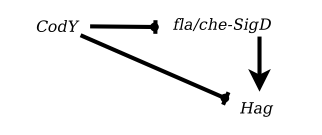
\includegraphics[scale=0.5]{wilkinson_reg_network.png}
\caption{Regulatory relationships. $Hag$ is the gene for $flagellin$, while $SigD$ encodes $\sigma^D$.}
\end{center}
\label{fig:}
\end{figure}

The paper focuses on measurements of $\sigma^D$. It attempts to infer the rates of binding of $fla/che$ repressors, unbinding of $fla/che$ repressors, and production of $\sigma^D$.

%Rather than describing regulatory relations in sentences, I'll relay Wilkinson's biochemical highlights in the following table. 
%
%$\left[
%\begin{tabular}{ >{}c<{} >{}c<{} >{}c<{} >{$}c<{$}}
% Name & Type of Molecule & suppresses & promotes& Is suppressed by & Is promoted by\\
% 
%flagellin & protein & -- & -- & -- & $\sigma^D$, {\it CodY} \\
%%
% $\sigma^D$ & protein & -- & -- & -- & -- \\
%%
% $\sigma^A$ & protein & -- & -- & -- & -- \\
%%
% {\it CodY}  & Type of Molecule & suppresses & promotes& Is suppressed by & Is promoted by\\
%\end{tabular} 
%\right]$

\section{The Model}
Since we're simulating a biochemical system, suppose there are $X_{j}(t)$ particles of type $j$ at time $t$, $j\in \{1 ... u\}$. These particles interact via a set of reactions $\mathcal{R}_{i}$, $i\in \{1 ... v\}$, with $\mathcal{R}_{i}$ consuming $p_{ij}$ particles of type $j$ and producing $q_{ij}$ particles of type $j$. Let $R_{i}(t)$ denote the number of reactions of type $i$ in $[0,t]$. I'll refer to these using the arrays $X(t)$, $P$, $Q$ and $R(t)$. Defining the matrix $S$ to be $Q^T-P^T$, the model says that $X(t) - X(0) = SR(t)$. Under some assumptions, the different reaction channels evolve independently, and $R_{i}(t)$ is a Poisson process with intensity $c_{i}\int_0^t \prod_{j=1}^u {{X_j(t)}\choose{p_{ij}}}$. %Define $h_{i}(c_{i}, X(t)) \equiv c_{i}\int_0^t \prod_{j=1}^u {{X_j(t)}\choose{p_{ij}}}$. 
The $c_{i}$'s are unknown.

Suppose $n$ reactions occur between time $0$ and time $T$. Suppose the $i$th one occurs at time $t_{i}$ and suppose it has type $\nu_{i}$. Define $t_0\equiv0$ and $t_{n+1}\equiv T$. When it comes to inference, the likelihood follows a competing-hazards model from continuous Markov chain theory.
%\footnote{At times, I choose to use equations that stand free of sentences. These I do not punctuate.}. 
%$$P(\nu, t|c) = \prod_{i=1}^n c_{\nu_{i}} \prod_{j=1}^u {{X_{j}(t_{i-1})}\choose{p_{{\nu_{i}}j}}}\exp\left(-c_{\nu_{i}}\int_0^T {{X_j(t)}\choose{p_{{\nu_{i}}j}}} dt\right)$$
%It contains the integral $\int_0^T {{X_j(t_{i-1})}\choose{p_{{\nu_{i}}j}}}dt$, which simplifies to $\sum_{i=0}^{n} (t_{i+1}-t_{i}) {{X_j(t_{i})}\choose{p_{{\nu_{i}}j}}}$. 
If the number of reactions of type $k$ is $r_k$, then the likelihood has a conjugate Gamma prior  
%$$P(\nu, t|c) = \prod_{k=1}^u \left\{ c_{k}^{r_k} 
%\left\{\prod_{j=1}^u { X_{j}(t_{i-1})\choose p_{kj}}^{r_k}\right\}\exp\left(-c_{k}\int_0^T \sum_j{X_j(t)\choose p_{kj}} \right)dt\right\}.$$  
%Still calling it the likelihood, Wilkinson omits the bracketed term $\prod_{j=1}^u { X_{j}(t_{i-1})\choose p_{kj}}^{r_k}$, probably because it does not involve $c$. Regardless, t
%The gamma distribution is conjugate for $c_k$, and setting independent priors 
$c_k\sim \Gamma(a_k, b_k)$, and the corresponding posteriors are independent with $c_k\sim \Gamma(a_k+r_k, b_k+\sum_{i=0}^{n} (t_{i+1}-t_{i}) {{X_j(t_{i})}\choose{p_{{\nu_{i}}j}}}$. This is an ideal scenario; missing data make inference more challenging.

\section{Inference}

In Wilkinson's data, not every reaction is recorded. Measurements are intermittent, with error, and only $\sigma^D$ or a fluorescent reporter gets measured. Conjugate priors cannot be used because, conditioned on discrete observations, the likelihood has no closed form--in fact, even evaluating the likelihood is not feasible. 
%Wilkinson says it better than I can: ``Consider ... observation of the system at discrete times. ... [T]he Markov process breaks up into a collection of independent bridge processes that appear not to be analytically tractable.'' %He goes on to mention alternative strategies, which include the MCMC scheme of \cite{Boys2008} and the approximation \cite{gillespie_CLE_2000} paired with inference via \EMK{cite more Wilkinson papers here.}
%For my own benefit: to produce a chain of samples from $P(\theta|D)$, using a proposal $q(\theta^*|\theta)$, accept with probability $\min \{1, A\}$ if $A=\frac{q(\theta|\theta^*)}{q(\theta^*|\theta)} \times \frac{P(\theta^*|D)}{P(\theta|D)}$. 
To adapt, the paper modifies likelihood-free methods from \cite{Marjoram23122003}. To make the mathematics easier to digest, I'll introduce first the predecessor and only then Wilkinson's method. 

Let $\theta$ include $c$, controlling the reaction rates, and $\tau$, controlling the scale of measurement error. Let $x$ denote the true state of the chain, but measured only at discrete times. The likelihood $P(x|\theta)$ cannot be evaluated. Let $\mathcal{D}$ be $x$ measured with error and possibly with missing data for some particle types. If we want to construct a Metropolis-Hastings scheme to sample from $P(x, \theta|\mathcal{D})\propto P( \theta)P(x| \theta)P(\mathcal{D}|x, \theta)$ using a proposal $f(\theta^*, x^*|\theta, x)$, it works out that the acceptance ratio must be the min of 1 and $$\frac{f(\theta^*, x^*|\theta, x)}{f(\theta, x|\theta^*, x^*)}\times 
\frac{ P( \theta)}{ P( \theta^*)} \times 
\frac{P(x| \theta)}{P(x^*| \theta^*)} \times
 \frac{P(\mathcal{D}|x, \theta)}{P(\mathcal{D}|x^*, \theta^*)}.$$ 

This genre of algorithms builds upon the fact that exact simulations from this model are possible, and also that measurement error helps soften the requirements on where the bridge process should begin and end. %In the model Wilkinson considers, $P(\mathcal{D}|x,\theta)$ is simple, but $P(x|\theta)$ is not feasible to compute. 
The insight from from \cite{Marjoram23122003} is that one can cancel the intractable term $ \frac{P(x| \theta)}{P(x^*| \theta^*)}$ by constructing a proposal that contains  $\frac{P(x^*| \theta^*)}{P(x| \theta)}$ as a factor. This factor arises if instead of drawing both $x^*$ and $\theta^*$ from simple out-of-the-box proposals, we draw only $\theta^*\sim f(\theta^*|\theta)$ and compute $x^*$ via simulation with parameters $\theta^*$. In the end result, the ratio of interest simplifies:
\begin{align*}
&\frac{f(\theta^*, x^*|\theta, x)}{f(\theta, x|\theta^*, x^*)}\times \frac{P(x| \theta)}{P(x^*| \theta^*)}\times \frac{ P( \theta)}{ P( \theta^*)}  \times \frac{P(\mathcal{D}|x, \theta)}{P(\mathcal{D}|x^*, \theta^*)}\\
&=\frac{f(\theta^*|\theta)}{f(\theta|\theta^*)}\times \frac{P(x^*| \theta^*)}{P(x| \theta)} \times \frac{P(x| \theta)}{P(x^*| \theta^*)} \times \frac{ P( \theta)}{ P( \theta^*)}\times \frac{P(\mathcal{D}|x, \theta)}{P(\mathcal{D}|x^*, \theta^*)}\\
&=\frac{f(\theta^*|\theta)}{f(\theta|\theta^*)}\times \frac{ P( \theta)}{ P( \theta^*)}\times \frac{P(\mathcal{D}|x, \theta)}{P(\mathcal{D}|x^*, \theta^*)}.
\end{align*}
To simplify further, use an independence sampler with the prior as a proposal, and the calculation reduces to $ \frac{P(\mathcal{D}|x, \theta)}{P(\mathcal{D}|x^*, \theta^*)}.$

If the measurement error is small, or $\mathcal{D}$ is high-dimensional, or both, this scheme leads to very high rejection rates, so it is not usable. Instead, you can break down $X$ and $\mathcal{D}$, adding only one data point at a time. The exact approach is best understood by referring to Algorithm 1. In broad strokes, the procedure alternates between generating large samples from $P(\theta, x_{t_{1:i}}|\mathcal{D}_{t_{1:i}})$, done via  likelihood-free MCMC, and folding in new data (incrementing $i$). To be clear, instead of running MCMC just once, in this method runs another five million steps through the sampler {\it for every time point in the dataset}. It isn't as bad as it sounds: for a sampler that runs only once, the chain will not mix without a sophisticated proposal, and constructing a usable proposal is often linear in the size of the data anyway. %This relies on the fact that the hidden state sequence is Markovian, i.e. that $P(x, \theta|\mathcal{D}) = \prod_t P(x_{t+1}, \theta|x_t, \mathcal{D})P(x_t, \theta|\mathcal{D})$. 
 

\begin{algorithm}[h]
\caption{ \label{seqMCMC} Wilkinson's sequence of MCMC Samplers}
Given a hidden continuous-time Markov process $\{x_t\}_{t=0}^T$ with: \\
\Indp \Indp
Unknown parameters $\theta$\\
Known initial state $x_0$\\
Data points $\mathcal{D}_{t_{i}}$ at times $t_{i}$, $i \in \{1, ... I\}$ \\
A simple, tractable error model $P(\mathcal{D}_{t_{i}}|x_{t_{i}}, \theta)$\\
A simulator for paths of $x$ given $\theta$ the process\\
A big array $B_0$ (Wilkinson uses length 1,000,000) of samples from a prior on $\theta, x_0$\\
Empty arrays $B_{i}$ of the same length\\
$\phantom{0}$\\
\Indm \Indm
For each time point (for $i \in \{1, ... I\}$), fill $B_{i}$ with samples from this Metropolis Hastings scheme:\\
\Indp\Indp
Initialize $(\theta, x_{t_{i}})$ \\
Until $B_{i}$ is full: \\
\Indp\Indp
Draw $(\theta^*, x_{t_{i-1}}^*)$ from $B_{i-1}$ or a KDE of its contents (note $t_0\equiv0$)\\
Using $(\theta^*, x_{t_{i-1}}^*)$, simulate up to $x_{t_{i}}^*$, the state at time $t_{i}$ \\
Set $A=\min(1, \frac{P(\mathcal{D}_{t_{i}}|x_{t_{i}}^*, \theta^*)}{P(\mathcal{D}_{t_{i}}|x_{t_{i}}, \theta)})$\\
With probability $A$, overwrite $(\theta, x_{t_{i}})$ with $(\theta^*, x_{t_{i}}^*)$\\
If the number of times through this loop exceeds 1000 ( for the burn-in) and equals one modulo five (for the thinning), add $(\theta, x_{t_{i}})$ to $B_{i}$\\
\Indm \Indm
\end{algorithm}


In any M-H scheme, the acceptance probability is either $1$ or the proposal ratio times the posterior ratio. For step $i$, the proposal ratio $\times$ posterior ratio can be expanded as follows:
$$ \frac{P(x_{t_{i}}^*| x_{t_{i-1}}^*,\theta^*\red{, \mathcal{D}_{t_{i-1}}})}{P(x_{t_{i}}| x_{t_{i-1}}, \theta \red{, \mathcal{D}_{t_{i-1}}})} 
\frac{P(x_{t_{i-1}}^*,\theta^*| \mathcal{D}_{t_{i-1}})}{P(x_{t_{i-1}}, \theta| \mathcal{D}_{t_{i-1}})}
\times 
\frac{P(x_{t_{i}}| x_{t_{i-1}}, \theta \red{, \mathcal{D}_{t_{i-1}}})}{P(x_{t_{i}}^*| x_{t_{i-1}}^*,\theta^*\red{, \mathcal{D}_{t_{i-1}}})}
\frac{ P(x_{t_{i-1}}, \theta| \mathcal{D}_{t_{i-1}})}{ P( x_{t_{i-1}}^*,\theta^*| \mathcal{D}_{t_{i-1}})}   
\frac{P(\mathcal{D}_{t_{i}}|x_{t_{i}}, \theta)}{P(\mathcal{D}_{t_{i}}|x_{t_{i}}^*, \theta^*)}.$$   
This shows how the compact form in Algorithm \ref{seqMCMC} arises. The Markov model would allow us to include or omit red terms at will, which is key: otherwise, the proposal, by design not conditioned on the data, would not cancel the intractable likelihood term. Note that using a KDE does not affect the ratio, because usually the kernel $K(\cdot|\cdot)$ is symmetric, so the extra term $\frac{K(\theta^*|\theta)}{K(\theta|\theta^*)}$ is just $1$.

\section{What could Wilkinson have done differently? Experiments and other research}


\subsection{Other work}
Wilkinson mentions many areas for future work in terms of biological applications for this method. In terms of new methodology, further work is needed to integrate data from microarrays or RNA-seq and to produce scalable methods that can process data on batches of cells.

To that end, there exist faster alternatives.  Some do not perform exact inference; a popular alternative is to approximate the process using a continuous-state diffusion process satisfying a certain SDE \cite{golightly2005bayesian,bayes_stoch_mod} or a linear approximation to such a diffusion process \cite{fearnhead2014inference}. Other non-exact methods include Approximate Bayesian Computation (ABC), which is compared with LF-MCMC in \cite{owen2014ABC_LF-MCMCcomparison}. Some alternative methods are exact, with a general theme of using approximations to generate good MCMC proposals. For examples, \cite{owen2014scalable} uses a parallelized ABC algorithm, \cite{milner2013moment} uses a method of moments scheme, and \cite{golightly2014smc_b_subtilis} explores several proposal-generating options, giving a particularly nice set of references in the process. Some proposal schemes condition on the desired end-points of the bridge process \cite{hobolth2009simulation}. The paper \cite{zechner2014scalable} is very similar to Wilkinson's, but inference is fast enough to use the method on batches of cells.

Non-MCMC alteratives exist, also. Like \cite{milner2013moment}, \cite{zechner2012moment} uses differential equations describing moments. Mean-field variational inference for Markov jump processes \cite{opper2008variational} works well even in small systems. James Rawlings' group has developed sampling algorithms that produce a semianalytical posterior distribution or likelihood over $\theta$, which they then optimize \cite{gupta2014comparison,srivastava_rawlings2014stoch_opt}. The papers \cite{bayer2015stoch_em,horvath2008parameter,daigle2012accelerated} are similar, carrying out EM with a sample average replacing the E-step expectation. Like Wilkinson's, these methods do not require evaluating intractable likelihoods. The paper  \cite{reinker2006parameter} gives a dozen references on the importance of stochasticity in regulatory networks. This area seems to have progressed rapidly starting around 2006: Reinker et al write in \cite{reinker2006parameter} that they are not
aware of methods that can cope with measurement error in systems with few molecules.

%To my surprise, though, I cannot find a paper using EM for discretely observed, infinite-state Markov jump processes of this type. As it was meant for motion tracking, \cite{fritsche2012online} assumes a form different from the Poisson processes that model chemical reactions, while work on codon substitution and epidemiology assumes a finite state space (e.g. \cite{jane_lange2013_vlad}).

\subsection{Summary of Experiments}

Wilkinson runs four main simulations. All tests are conducted using synthetic data on only one vector of true parameters. The first three iterate through successively more difficult and realistic measurement models:
\begin{itemize}
\item First experiment: observe $\sigma^D$  directly
\item Second experiment: observe $Hag$ rather than $\sigma^D$
\item Third experiment: observe only a fluorescent reporter
\end{itemize}

The fourth shows that a naive model, assuming the fluorescent reporter protein is proportional to the protein of interest, leads to strong and incorrect claims in the posterior probabilities. 

\subsubsection{Some details needed to reproduce experiments}
Wilkinson describes a twelve-reaction regulatory model for these chemicals, spelling it out in table 1, and he lists three scientifically important reaction rates that, for tests of the inference method, will be treated as a ``ground truth.'' The prior distributions cover 4 orders of magnitude, and they are uniform on a log scale. The experiment assumes $D_t$ is the number of molecules observed with Gaussian error of standard deviation 10 molecules. %\EMK{Gaussian noise for integer data? Could do Bin($p=0.5, n=40$). What is the physical mechanism behind the measurement error?} 
The initial state of the cell is assumed known \EMK{but does he specify it?}, and observations occur every 5 minutes (300 seconds) for 2 hours (7200 seconds). 

%Wilkinson says ``1,000,000 particles were used, together with a burn-in of 1,000 iterations and a thin of 5[.]''
% \EMK{He never defines particles, so pending further reading, my best guess is that this means he starts with 1e6 samples from the prior, carrying each one forward. Not sure how the burn-in fits in.} 

%He also repeats this experiment, altering the measurement process so that it relies on a proxy for $\sigma^D$, a fluorescent protein (GFP). He performs inference by a) plugging GFP levels into the algorithm as if they were exactly proportional to $\sigma^D$ and b) including the production and decay of GFP in the biochemical model. He concludes that plugging in GFP for $\sigma^D$ leads to strong, incorrect posteriors, but that the full model is still useful.

 \subsection{Critique of experiments}
Some authors \cite{protein_interaction} claim that reaction rates range over seven orders of magnitude, but Wilkinson's prior covers only four orders of magnitude. Furthermore, it is centered around the ground truth. What happens when the log-space mean of the prior is not near the true values? Wilkinson recognizes prior selection as an issue, citing \cite{liebermeister2005biochemical}, but declines to pursue it, with an implicit claim that reasonable choices of prior will not jeopardize the method. 

Wilkinson also treats parameters as known except for the three parameters of interest. How well does this method work when the rest of the reaction rates must also be inferred, or when the measurement error variance must be inferred?

%I am no expert on dynamical systems, but I would add that in isolation, parameter inference does not seem to contribute much to our understanding of these systems. A modeling endeavor of this sort should culminate in successful predictions; what will Wilkinson predict here? Systems with multiple stable modes corresponding to bacterial behaviors? Previously unknown biochemical interactions? Fruitful sites to target antibiotics that disrupt bacterial metabolism? \EMK{Update: another of Wilkinson's papers says that parameter inference is essential to larger modeling projects \cite{golightly2005bayesian}. There is a discussion of this reverse engineering in \cite{Bower:2004:CMG:1197014}.}

%\begin{itemize}
%\item His likelihood-free MCMC scheme applies to any hidden, discretely observed continuous Markov process. It also can be used for multiple time-series $\mathcal{D}^1, ..., \mathcal{D}^p$ by using posteriors from one as priors for the next.
%\item This method can fuse data from two bacterial strains, one missing a certain gene, by using posteriors from one experiment as priors for the next. It can also accomodate multiple fluorescent ``reporters'' for different molecules.
%\item Unsolved problems include scaling the method up to process data on batches of cells integrating data from microarrays or RNA-seq.
%\end{itemize}

%I also have some ideas.
%\begin{itemize}
%\item For scaling, could an EM algorithm handle the missing data more quickly?
%\item Do you really need such a large sample for every intermediate step? 
%\item To avoid the first T-1 runs of the sampler in a setting with  could you build proposal distributions using variational methods?
%\item Could I build BEMC around this?
%\end{itemize}

\begin{align*}
\end{align*}
\begin{align*}
\end{align*}
\begin{align*}
\end{align*}
\begin{align*}
\end{align*}

%\texttt{code snippet}
%
%\begin{algorithm}[h]
%\caption{ }
%Do things\\
%Loop:\\
%\Indp
% Do this again and again\\
%\end{algorithm}

%\begin{figure}[h!]
%\begin{center}
%\includegraphics[height=4in,width=6in]{filename.pdf}
%\caption{}
%\end{center}
%\label{fig:}
%\end{figure}

%$\left[
%\begin{tabular}{ >{$}c<{$} >{$}c<{$}}
% 1 & -\phi_1\\
% -\phi_1 & 1
%\end{tabular} 
%\right]$

%==== Bib files and style =======
\bibliographystyle{splncs}
\bibliography{prelim_biblio}
\end{document}
